% This material is copyright Simon Dobnik and made available under the
% Creative Commons Attribution 4.0 International License (CC-BY-SA)
% license http://creativecommons.org/licenses/by-sa/4.0/
% 
% Email: simon.dobnik@gu.se
% Web: http://dobnik.net/simon/teaching/shared/LT2112-formling/


\documentclass{beamer}

\usepackage{graphicx,hyperref,lingmacros,qtree,avm,fullname} 




\logo{
\includegraphics[height=0.5cm]{pics/GU-logo.pdf}} 
\newcommand{\bblue}[1]{{\usebeamercolor[fg]{frametitle}{#1}}}


\definecolor{links}{HTML}{2A1B81}
\hypersetup{colorlinks,linkcolor=,urlcolor=links}

\setbeamertemplate{footline}[frame number]

\resetcounteronoverlays{enums}

\AtBeginSection[]
{
\begin{frame}[plain]

{\huge\bblue{\insertsectionhead}}

\end{frame}
}



\avmfont{\sc}
\avmsortfont{\scriptsize\it}

\renewcommand{\rmdefault}{\sfdefault}
\renewcommand{\scdefault}{\sfdefault}



\newcommand{\lb}[1]{[$_{\textsf{#1}}$} 
\newcommand{\ibar}[1]{$\overline{#1}$} 








\newcommand{\trace}{\underline{\hspace{0.5cm}}}





\title[Syntax]{L6: Syntax III - Dependencies}

\author[Dobnik]{Simon Dobnik \\ 
Department of Philosophy, Linguistics and Theory of Science
} 

\date{September 24, 2015}





\begin{document}





\frame{\titlepage}





\frame{

\frametitle{Outline}

\tableofcontents

}





\section{Local dependencies: NPs}

\frame{

\frametitle{From verbal arguments to NPs}

Previously, \ldots

\begin{itemize}

\item verbs are predicate relations that take various arguments of entities or events;

\item they restrict their arguments by a thematic role: Agent, Experiencer, Goal, Source, Location, Theme.

\end{itemize}

\pause \bigskip


How can we tell in a sentence what NP fulfils what role?

\pause

\begin{itemize}

\item Structural relations

\item Morphological marking (case)

\end{itemize}


}





\subsection{Identifying NPs}

\frame{

\frametitle{Identifying NPs: structural relations}

\Tree [.TP [.NP [.N George\\\bblue{Agent} ] ] [.VP [.V gave ] [.NP [.D a ] [.N present\\\bblue{Theme} ] ]  [.PP [.P to ] [.NP [.N Lydia\\\bblue{Goal} ] ] ] ] ]

}





\frame{

\frametitle{Identifying NPs: structural relations}

\Tree [.TP [.NP [.N George\\\bblue{Agent} ] ] [.VP [.V gave ]  [.NP [.N Lydia\\\bblue{Goal} ] ] [.NP [.D a ] [.N present\\\bblue{Theme} ] ] ] ]

}





\begin{frame}

\frametitle{Identifying NPs: structural relations}

\begin{itemize} 
\item The number of slots that an NP can occupy is limited

\item They are structurally defined

\item The slots are said to define \bblue{grammatical relations} of an NP: subject, direct and indirect object, infinitival complement, sentential complement,\ldots

\end{itemize}

\end{frame}





\frame{

\frametitle{Identifying NPs: morphological marking with Case}

Subject-object case marking in English


\eenumsentence{
	\item \bblue{She} saw \bblue{him}.
	\item \bblue{He} saw \bblue{her}.
	\item \bblue{It} broke \bblue{it}.
	}

}





\frame{

\frametitle{Identifying NPs: morphological marking with Case}

Japanese \cite{Carnie:2007aa}, p.296: Subject: \bblue{-ga}, Direct object: \bblue{-o}, Indirect-object$|$Adjuncts: \bblue{-ni}


\eenumsentence{
	\item \shortex{3}{Asako-ga & ronbun-o & kai-ta.}
	{Asako-{\sc subj} & article-{\sc d-obj} & wrote-{\sc past}}
	{``Asako wrote the article.''}
	\item \shortex{3}{Etsuko-ga & heya-ni & haittee-kita.}
	{Etsuko-{\sc subj} & room-{\sc i-obj} & in-came.}
	{``Etsuko came into the room.''}
	}
}





\frame{

\frametitle{Identifying NPs: complex case systems (Finish)}

\begin{center}
\footnotesize
\begin{tabular}{l l l}
\hline
\bblue{Case} & \bblue{Example} & \bblue{English equivalent} \\
\hline
nominatiivi & talo & house \\ 	
genetiivi & talon & of (a) house \\
essiivi & talona & as a house \\
partitiivi & taloa & house (as an object) \\
translatiivi & taloksi & to a house \\
inessiivi & talossa & in (a) house \\
elatiivi & talosta & from (a) house \\
illatiivi & taloon & into (a) house \\
adessiivi & talolla & at (a) house \\
ablatiivi & talolta & from (a) house \\
allatiivi & talolle & to (a) house \\
abessiivi & talotta & without (a) house \\
komitatiivi & taloineni & with my house(s) \\
instruktiivi & (talon) & with (a) house 
\end{tabular}
\end{center}

\pause

Also includes other semantic properties. Examples from \href{http://www.cs.tut.fi/~jkorpela/finnish-cases.html}{\bblue{here}}.

}





\frame{

\frametitle{Representing Case in FSs}


Case as a head feature on nouns


\begin{itemize}

\small

\item N[head=[agr=[num=sg,pers=3,case=acc,gen=fem]]] $\rightarrow$ her

\item N[head=[agr=[num=sg,pers=3,case=nom,gen=masc]]] $\rightarrow$ he

\item \pause NP[head=A] $\rightarrow$ N[head=A]

\end{itemize}

\bigskip \pause

From arguments of lexical predicates to structural positions 

\begin{itemize}

\item V[head=[agr=[num=sg,pers=3]],subcat=[obj,subj]] $\rightarrow$ saw

\item \pause VP[head=A,subcat=Rest] $\rightarrow$ V[head=A,subcat=[obj$|$Rest]] NP[head=[agr=[case=acc]]]


\item \pause TP[subcat=[]] $\rightarrow$ NP[head=[agr=[num=N,pers=P,case=nom]]] VP[head=[agr=[num=N,pers=P,subcat=[Last]]]]

\end{itemize}

}





\begin{frame}[fragile]

\frametitle{Representing Case in FSs}



\begin{itemize}

\small

\item \verb+N[head=[agr=[num=sg,pers=3,case=acc,gen=fem]]]+ \\ \verb+   -> 'her'+

\item \verb+N[head=[agr=[num=sg,pers=3,case=nom,gen=masc]]]+ \\ \verb+   -> 'he'+

\item \verb+NP[head=A] -> N[head=A]+

\item \pause \verb+V[head=[agr=[num=sg,pers=3]],subcat=trans] -> 'saw'+

\item \verb+VP[head=A] ->+ \\ \verb+   V[head=A,subcat=trans] NP[head=[agr=[case=acc]]]+

\item \pause \verb+TP -> NP[head=[agr=[num=?num,pers=?pers,+ \\ \verb+   case=nom]]] VP[head=[agr=[num=?num,pers=?pers]]]+

\end{itemize}

\end{frame}





\subsection{Alternations of argument structure}

\subsubsection{Passive}


\frame{

\frametitle{Alternations of argument structure: Passive}



A mismatch between thematic structure and structural relations:


\eenumsentence{
	\item George kissed Lydia. (\bblue{Active})
	\item Lydia was kissed by George. (\bblue{Passive})
	\item Lydia was kissed.
	}

\pause \bigskip

Changes the argument structure of the verb. 
\begin{itemize}
\item kiss: $\langle$Agent, Theme$\rangle$
\item kissed: $\langle$Theme$\rangle$
\end{itemize}

\bigskip

The \bblue{Theme} argument is realised as a subject!

}





\subsubsection{Un-accusatives}

\frame{

\frametitle{Un-accusatives: inherently passive verbs}

\bblue{Not all intransitive verbs are the same.}


\eenumsentence{
	\item George \bblue{danced} at the barn.
	\item George \bblue{arrived} at the barn.
	}

\pause

\eenumsentence{
	\item dance: $\langle$Agent$\rangle$
	\item arrive: $\langle$Theme$\rangle$
	}

\pause \bigskip

\bblue{We cannot ``force'' \bblue{arrive} to take another \bblue{Theme} argument.}


\eenumsentence{
	\item George danced a jig.
	\item *George arrived a barn.
	}

}





\frame{

\frametitle{Un-accusatives: inherently passive verbs}

\bblue{Have/Be auxiliary alternation in German, Italian\ldots}

\eenumsentence{
	\item Georg \bblue{hat} getanzt. \\ George has danced
	\item Georg \bblue{ist} angekommen. \\ George is arrived
	}

\pause \bigskip

An alternating example:

\eenumsentence{
	\item George sank the boat.
	\item The boat sank.
	\item The boat was sunk by George.
	}


\bigskip

The \bblue{Theme} argument is realised as a subject!

}





\subsection{Arguments in non-finite clauses}

\subsubsection{Raising}

\frame{

\frametitle{Arguments in non-finite clauses: Raising}

Arguments are realised \bblue{locally} to the predicate that assigns it.


\eenumsentence{
	\item *\lb{TP}I want \underline{George} \lb{CP} that \underline{\hspace{0.5cm}} danced] ].
	\item *\lb{TP}\underline{Lydia} thinks \lb{CP} that \underline{\hspace{0.5cm}} danced] ].
	}
 
\pause \bigskip

However, with some non-finite complements\ldots


\eenumsentence{
	\item \lb{TP}\underline{George} is likely \lb{TP}\underline{\hspace{0.5cm}} to dance] ].
	\item \lb{TP}\underline{It} is likely \lb{CP} that George will dance] ].
	\item \lb{TP}\lb{CP}\underline{That George will dance}] is likely ].
	}

\pause

\eenumsentence{
	\item is-likely: $\langle$Event$\rangle$
	\item dance: $\langle$Agent$\rangle$
	}

}





\frame{

\frametitle{Observations about raising}

\begin{itemize}

\item If the embedded verb is not tensed:\\
	\begin{itemize}
		\item its argument (\bblue{Agent}) becomes the subject of the main verb.
	\end{itemize}

\pause

\item If the embedded verb is tensed:\\
	\begin{itemize}
		\item The subject must be filled with a non-thematic ``it''
		\item The subject must be filled with the \bblue{Event} argument.
	\end{itemize}
\end{itemize}

}











\frame{

\frametitle{Conclusions on raising}


All NP arguments \bblue{must be} licensed as \bblue{grammatical relations}.


\enumsentence{*It was kissed Lydia.}



\pause

\bigskip

Non-finite clauses \bblue{cannot} license subjects.

\pause

\bigskip

Finite clauses \bblue{must} license subjects.

}





\subsubsection{Control}

\frame{

\frametitle{Raising and Control}

Not all non-finite clauses are the same.

\eenumsentence{
	\item \pause \underline{George} is likely \lb{TP}\underline{\hspace{0.5cm}} to dance]. \\ is-likely: $\langle$Event$\rangle$ \\ dance: $\langle$Agent$\rangle$ 	\item \pause George is reluctant \lb{TP} PRO to dance]. \\ reluctant: $\langle$Agent, Event$\rangle$ 	\item \pause George wants \underline{Lydia} \lb{TP}\underline{\hspace{0.5cm}} to dance]. \\ want: $\langle$Agent, Event$\rangle$ $|$ $\langle$Agent, Theme$\rangle$ 	\item \pause George persuaded Lydia \lb{TP} PRO to dance]. \\ persuade: $\langle$Agent, Theme, Event$\rangle$ 	}

}





\frame{

\frametitle{There are really ARE two subjects}

The subject of the main verb cannot be replaced by ``it'' or a ``that'' clause if ``George'' gets licensed in the complement clause.

\bigskip

\eenumsentence{
	\item *\lb{TP}\bblue{It} is reluctant \lb{CP}that \bblue{George} will dance].
	\item *\lb{TP}\lb{CP} \bblue{That George will dance}] is reluctant].
	}

}





\frame{

\frametitle{Some TPs have a non-pronounced subject pronoun}



PRO (aka `the big pro')

\bigskip

PRO may have various antecedents.

\pause


\eenumsentence{
	\item George was reluctant \lb{TP}PRO to meet at the barn].\\
	PRO = \{George, Lydia, Simon, \dots\}
	\item \pause PRO to buy flowers, go to a florist. \\
	PRO = \{ ? \}
	\item \pause George knows that it is essential PRO to be well behaved. \\
	PRO = \{ George, ? \}
	}


}





\frame{

\frametitle{How is PRO's reference assigned?}

A property of lexical entries?

\eenumsentence{
	\item Lydia$_i$ instructed George$_j$ PRO$_{*i/j}$ to behave.
	\item George$_j$ promised Lydia$_i$ PRO$_{*i/j}$ to behave.
	}

\pause

But\ldots

\eenumsentence{
	\item George$_j$ begged Lydia$_i$ PRO$_{i/*j}$ to buy an iPad.
	\item George$_j$ begged Lydia$_i$ PRO$_{i*/j}$ to be allowed to use it.
	}
}





\frame{

\frametitle{Further reading}

Advanced: presupposes familiarity with a particular syntactic theory

\bigskip

\cite{Carnie:2007aa} Chapters 10 (DP movement) and 13 (Raising, Control and Empty Categories).

\bigskip

\cite{Dalrymple:2001aa} Chapters 8 (Argument structure and mapping theory) and 12 (Functional and anaphoric control). 
\bigskip

Practical implementation:

\bigskip

\cite{Bird:2009ab}: \href{http://www.nltk.org/book/ch09.html}{Chapter 9} Building Feature Based Grammars.


}





\frame{

\frametitle{Intermediate summary}

So far we discussed that\ldots

\begin{itemize}

\item \pause Verbs select for arguments or $\theta$-roles (lexical dependencies).
\item \pause Lexical dependencies are represented in syntax:\\ syntactic dependencies or GRs.

\item \pause A certain $\theta$-role is not always represented as the same GR.

\item \pause The dependencies must be \bblue{local to the verb} - within a TP.

\end{itemize}

\pause

\bigskip

But there are some dependencies that are \bblue{non-local}.

}





\section{Long distance dependencies}


\subsection{Topicalisation}

\frame{

\frametitle{Topicalisation in English}

Certain constituents can be \bblue{fronted} or \bblue{extracted}.

\pause

\eenumsentence{
	\item\label{topic:a} \bblue{NP:} \underline{George}, I hate \trace.
	\item \pause \bblue{AP:} \underline{Grateful}, George will never be \trace.
	\item\label{topic:c} \pause \bblue{PP:} \underline{To Lydia}, George gave a present \trace.
	\item\label{topic:d} \pause \bblue{CP:} \underline{That George would become famous}, Lydia did not expect \trace.
	\item \pause \bblue{VP:} ?\underline{To catch a mouse}, we convinced George \trace.
	}

\pause \bigskip

Fronted constituents are already marked for GRs: \\Object (\ref{topic:a}), Indirect Object (\ref{topic:c}).

}





\frame{

\frametitle{Syntax of topicalised phrases}

The topicalised phrase must be ``higher'' than the subject.

\pause \bigskip

\enumsentence{
\Tree [.CP [.NP [.N George ] ] [.TP [.NP [.N I ] ] [.VP [.V like ] [.NP ]  ] ] ]
}

}





\frame{

\frametitle{Long-distance topicalisation}

The topicalised phrase may be extracted from \bblue{complement clauses}.

\pause

\eenumsentence{
	\item \lb{CP}\lb{NP}George], \lb{TP} I think \lb{CP} that \lb{TP }Lydia saw \trace]]]].
	\item \pause \lb{CP}\lb{AP}Grateful], \lb{TP} I think \lb{CP} that \lb{TP }George will never be \trace]]]].
	\item \pause \lb{CP}\lb{PP}To Lydia], \lb{TP} I think \lb{CP} that \lb{TP }George gave a present \trace]]]].
	\item \pause \lb{CP}\lb{CP}That George will become famous], \lb{TP} I think \lb{CP} that \lb{TP }Lydia never expected \trace]]]].
	\item \pause ?\lb{CP}\lb{VP}To catch a mouse], \lb{TP}I think \lb{CP} that \lb{TP }we convinced George \trace]]]].
	}

}





\frame{

\frametitle{Some restrictions}

Not possible with every matrix verb


\eenumsentence{
	\item \lb{CP}\lb{NP}George], \lb{TP} I \bblue{think} \lb{CP} that \lb{TP }Lydia saw]]]].
	\item *\lb{CP}\lb{NP}George], \lb{TP} I \bblue{whispered} \lb{CP} that \lb{TP }Lydia saw]]]].
	}

\pause \bigskip

Not possible to extract from CPs that are subjects

\enumsentence{*\lb{CP} \lb{NP} George], \lb{TP}\lb{CP} that Lydia saw \trace] surprised me]].}

}





\frame{

\frametitle{Some restrictions}

Extracting from adjuncts only possible if they are not tensed

\eenumsentence{
	\item \lb{CP}\lb{NP}This garden], \lb{TP} George enjoys sleeping \lb{PP}in \trace]]].
	\item\label{relclause} *\lb{CP}\lb{NP}Lydia] Simon thinks \lb{CP} that George slept \lb{CP}when he called \trace]]].
	}

}





\subsection{Relative clauses}

\frame{

\frametitle{Relative clauses}

An XP modified by a tensed adjunct CP.

\bigskip

The \bblue{wh-}constituent (the relative pronoun) is fronted within the adjunct.



\bigskip

\eenumsentence{
	\item \bblue{NP:} \underline{a person} \underline{who(m)} I saw \trace 
	\underline{a person} \underline{whose picture} George found \trace
	\item \bblue{PP:} \underline{a person} \underline{to whom} George gave a present \trace
	\item \bblue{AP:} \underline{a person} \underline{envious of whom} I get easily \trace
	\item \bblue{AdvP:} \underline{the place} \underline{where} we met \trace
	\underline{the hour} \underline{when} we argued \trace
	}
}





\frame{

\frametitle{Pied piping}

If a relative pronoun appears in a constituent, the entire constituent is fronted.

\eenumsentence{
	\item the person \underline{whose garden} George visited \trace. \\ *the person \underline{whose} George visited garden \trace.
	\item \pause the person \underline{the cat of whom} I saw \trace in the garden. \\ *the person \underline{of whom} I saw the cat \trace in the garden.
	\item \pause the cat \underline{the colour of the fur of which} Lydia likes \trace. \\ *the cat \underline{of which} Lydia likes the colour of the fur \trace.
	}

}





\frame{

\frametitle{Pied Piper of Hamelin}

\begin{center}
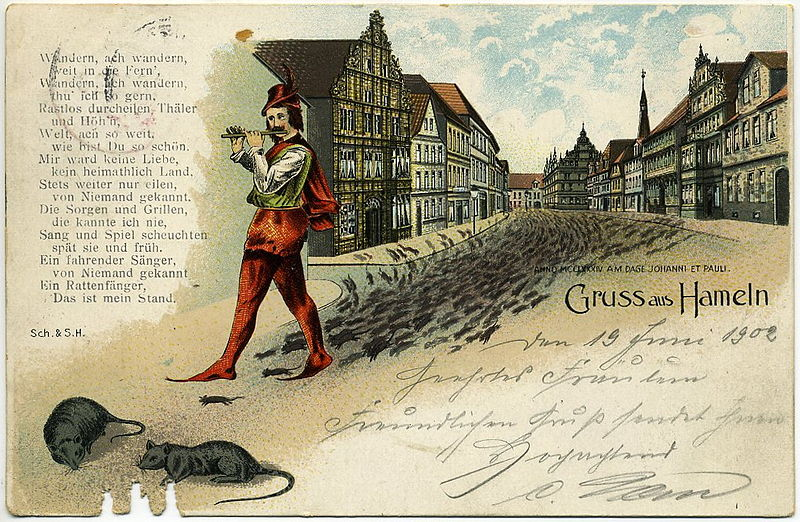
\includegraphics[scale=0.66]{pics/Hameln}

From Wikipedia, also \href{http://en.wikipedia.org/wiki/Pied_Piper_of_Hamelin}{article}
\end{center}

}





\frame{

\frametitle{Relative clauses without a relative pronoun}


\eenumsentence{
	\item I have seen the spacecraft \bblue{which} George owns.
	\item I have seen the spacecraft \bblue{that} George owns.
        \item I have seen the spacecraft George owns.
	\item\label{dfcompf} \pause *I have seen the spacecraft \bblue{which that} George owns.
}


\bigskip

(\ref{dfcompf}): Doubly Filled Comp Filter\\
*\lb{CP} wh-XP that]


}





\frame{

\frametitle{Syntax of relative clauses}


\enumsentence{ \Tree [.NP [.D a ] [.N person ] [.CP [.NP [.N whom ] ] [.TP [.NP [.N George ] ] [.VP [.V saw ] [.NP ] ] ] ] ] 
}

}





\frame{

\frametitle{Same extraction constraints as topicalisation}


\eenumsentence{
	\item \underline{George}, I think that Lydia saw \trace.\\
	a person \underline{who} you think that Lydia saw \trace
	\item *\underline{George}, I whispered that Lydia saw \trace. \\
	*a person \underline{who} you whispered that Lydia saw \trace
	\item \pause *\underline{George}, \lb{CP}that Lydia saw \trace] surprised me. \\
	*a person \underline{who} \lb{CP} that Lydia saw \trace] surprised me
	\item \pause \underline{This garden}, George enjoys sleeping \lb{PP}in \trace]. \\
	this garden \underline{which} George enjoys sleeping \lb{PP}in \trace]
	\item \pause *\underline{Lydia} Simon thinks that George slept \lb{CP} when he called \trace].\\
	*a person \underline{who} Simon thinks that George slept \lb{CP} when he called \trace]
	}

}





\subsection{Wh-questions}

\frame{

\frametitle{Wh-questions}

A constituent containing a \bblue{wh-}pronoun is fronted.

\bigskip

The auxiliary precedes the subject as with (yes/no) questions.

\bigskip


\eenumsentence{
	\item \bblue{NP:} \underline{Who} does George like \trace?
	\item \bblue{PP:} \underline{To whom} did George give a present \trace?
	\item \bblue{AdvP:} \underline{When} did George leave the stage \trace?\\
	\underline{Where} did George go \trace?
	\item \bblue{AP:} \underline{How lazy} is George?
	}

}





\frame{

\frametitle{Pied piping}

Embedded \bblue{wh-}pronouns front the entire phrase:


\eenumsentence{
	\item \underline{Whose garden} did you visit \trace? \\ *\underline{Whose} did you visit \trace garden?
	\item \pause \underline{Whose brother's garden} did you visit \trace? \\ *\underline{Whose} did you visit \trace brother's garden?
	\item \pause \underline{In which garden} did George sleep \trace? \\ *\underline{In which} did George sleep \trace garden?
	\item \pause *\underline{The colour of the fur of which cat} does \\Lydia like \trace? \\ *\underline{Of which cat} does Lydia like the colour of the fur \trace? \\
	\underline{Which cat} does Lydia like the colour of \trace?
	}



}





\frame{

\frametitle{How many \bblue{wh-}phrases can be fronted?}



\eenumsentence{
	\item \bblue{English:}\\
	*\underline{Who} \underline{what} \trace said \trace?
	\item \bblue{French:} \\
	*\underline{Qui} \underline{quoi} \trace {} fait \trace? - who what does
	\item \pause \bblue{Polish:} \\
	\underline{Kto} \underline{co} \trace {} robi \trace? - who what does
	\item \pause \bblue{Hungarian:} \\
	\underline{Ki} \underline{m\`{i}t} \trace {} latott \trace? - who what saw
	}

\bigskip

From \cite{Haegeman:1994aa}, p.504.

}





\frame{

\frametitle{Is \bblue{wh-}fronting required?}


\eenumsentence{
	\item *George saw what?
	\item George so WHAT?
	}

\pause



\eenumsentence{
	\item\label{whinsitua} \shortex{5}{John-ga & dare-o & butta & ka & siranai.}
	{John & who & hit & Q & {know not}}
	{`I don't know who John hit.' (Japanese)}
	\item\label{whinsitub} \shortex{5}{Wo & xiang-zhidao & Lisi & mai-le & sheme}
	{I & wonder & Lisi & bought-aspect & what}
	{`I wonder what Lisi bought.' (Chinese)}
	}

\bigskip

From \cite{Haegeman:1994aa}, p.497--498.

}





\frame{

\frametitle{The auxiliary in \bblue{wh-}questions}

\bblue{The auxiliary appears in T.}

\enumsentence{\lb{TP}\lb{NP}George] \lb{T}does] \lb{VP}like playing in the garden]].}

\bigskip \pause

\bblue{In questions the auxiliary precedes the subject `George'.}

\eenumsentence{
	\item Does \lb{TP}\lb{NP}George] \lb{VP} like playing in the garden]]?
	\item What does \lb{TP}\lb{NP}George] \lb{VP}enjoy doing]]?
	}

\bigskip \pause

\bblue{But not in the embedded questions.}


\eenumsentence{
	\item I wonder what George has done now.
	\item *I wonder what has George done now.
	}
}





\frame{

\frametitle{Syntax of \bblue{wh-}questions}


\enumsentence{\Tree [.CP [.Wh who ] [.C does ] [.TP [.NP [.N George ] ] [.VP [.V like ] [.NP ] ] ] ]
}

}





\frame{

\frametitle{\bblue{Wh-}pronouns can be extracted from embedded clauses}

\eenumsentence{
	\item \lb{CP}\underline{Who(m)} did you think \lb{CP}\bblue{that} Lydia kissed \trace]]?
	\item \lb{CP}\underline{Who(m)} did you think \lb{CP} Lydia kissed \trace]]?	
	}

}





\frame{

\frametitle{Constraints on wh-extraction}

\bblue{\Large 1.} Extraction is not possible when the \bblue{wh-}pronoun is a subject preceded by a complementiser `that' (that-trace effect):


\eenumsentence{
	\item *\lb{CP}\underline{Who} do you think \lb{CP}\bblue{that} \trace kissed Lydia]]?
	\item \lb{CP}\underline{Who} do you think \lb{CP} \trace kissed Lydia]]?
	}

\pause \bigskip

But in Italian it is okay.

\enumsentence{\shortex{6}{\underline{Chi} & credi & che & \trace & {} &venga?}
{who & think-you & that & {} & comes}
{``Who do you think is coming?''}}


}





\frame{

\frametitle{Constraints on \bblue{wh-}extraction}

\bblue{\Large 2.} Extraction from complement CPs is okay, but not if the CP is within an NP.

\eenumsentence{
	\item \underline{What} did George claim \lb{CP} that he caught \trace {} in the garden]?
	\item *\underline{What} did George make \lb{NP} the claim \lb{CP} that he caught \trace {} in the garden]?
	}
}





\frame{ 

\frametitle{Constraints on \bblue{wh-}extraction}

\bblue{\Large 3.} Extracting from subject CPs is not possible (as seen earlier).

\enumsentence{*\underline{Who} did \lb{CP} that Lydia saw \trace] surprised George?}


}





\frame{

\frametitle{More constraints on \bblue{wh-}extraction }

\bblue{\Large 4.} Extracting multiple \bblue{wh-}constituents is not possible.

\eenumsentence{
	\item *\underline{Who} did you think \lb{CP} \underline{what} \trace {} saw \trace]?
	\item \underline{Who} did you think \lb{CP} \trace {} saw what]?
	}

\bigskip \pause

This explains the difference between non-tensed and tensed adjuncts noted before.

\eenumsentence{
	\item  \underline{Where} does George enjoy sleeping \lb{PP}in \trace]? 
	\item *\underline{Who} does Simon think that George slept \lb{CP} when he called \trace]?
	}

}





\frame{

\frametitle{More constraints on \bblue{wh-}extraction}

\bblue{\Large 5.} Lexical constraints of verbs (as seen earlier)

\enumsentence{
\item *\underline{Who} did you whisper that Lydia saw \trace?
}

}





\frame{

\frametitle{A brief explanation of this data}

\begin{itemize}

\item  Structural relations between the extracted element and the site of extraction matter. (e.g. subject CPs).

\item \pause The extracted element and the site of extraction are linked.

\item \pause In long distance dependencies, the extraction may cross a CP, but only one: \\  \lb{CP}\underline{Who} do you think \lb{CP} \trace {} that George claimed \lb{CP} \trace {} that Lydia saw \trace]]]?

\item \pause NPs do not allow such paths (no extraction from \lb{NP}\lb{CP}here]].

\end{itemize}


}





\frame{


\frametitle{Gap threading with FS}


\begin{itemize}

\small

  \item V[head=[agr=[num=inf,pers=inf],subcat=[obj,subj]] $\rightarrow$ like

  \item \pause VP[head=[agr=[num=inf,pers=inf],subcat=Rest,\bblue{gap=G}] $\rightarrow$ V[[head=[agr=[num=inf,pers=inf],subcat=[\bblue{G}$|$Rest]]

  \item \pause TP[head=[agr=[num=N,pers=P]],subcat=[],\bblue{gap=G}] $\rightarrow$ NP[head=[agr=[num=N,pers=P,case=nom]]] VP[head=[agr=[num=inf,pers=inf],subcat=[Last]],\bblue{gap=G}]

  \item NP[head=A] $\rightarrow$ N[head=A]

  \item \pause  CP[focus=\bblue{G}] $\rightarrow$ Wh[gr=\bblue{G},member(\bblue{G},[subj,obj,indo,adj])] C[head=A] TP[head=A,\bblue{gap=G}]

  \item Wh[gr=obj] $\rightarrow$ who $|$ whom

  \item C[head=[agr=[num=3,pers=sg] $\rightarrow$ does

\end{itemize}

}





\frame{

\frametitle{Gap threading with FS}

feat01.fcfg

}





\frame{

\frametitle{Syntax of \bblue{wh-}questions}

\begin{center}
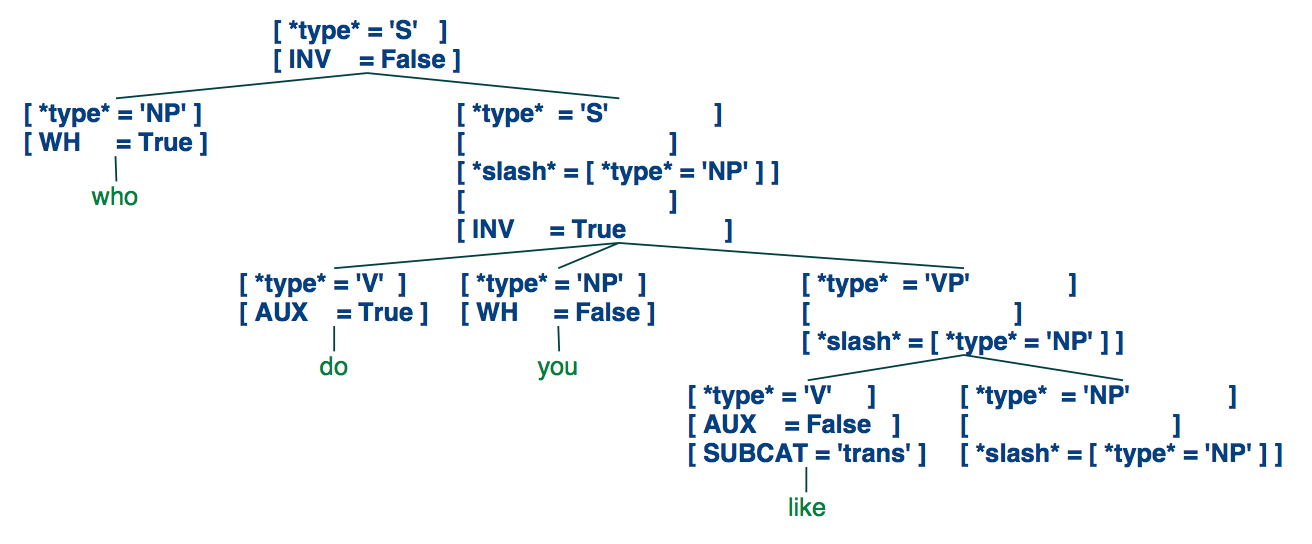
\includegraphics[width=\textwidth]{pics/gap-threading2.png}
\end{center}

}





\frame{

\frametitle{Further reading}

Advanced: presupposes familiarity with a particular syntactic theory

\bigskip

\cite{Dalrymple:2001aa}: Chapter 14 (Long-distance dependencies). 
\bigskip

\cite{Carnie:2007aa}: Chapter 10 (\emph{Wh-}movement).

\bigskip

Practical implementation:

\bigskip

\cite{Bird:2009ab}: \href{http://www.nltk.org/book/ch09.html}{Chapter 9} Building Feature Based Grammars.

}





\begin{frame}[allowframebreaks]{References}

\small


\bibliographystyle{fullname}
\bibliography{bibliography}

\end{frame}


\end{document}



